\subsection{Summary View}
\label{sec:allPairs}
% outline:
%  - how to identify the sensitivity of pairs
We can only focus on one individual example at a time for detailed analysis using the combination of all previously discussed views. As a result, how to select a pair of sentences of interests from the development or test dataset, which consists of close to $10k$ examples, is an obvious challenge.
% - what is the interesting pairs
In addition, the experts also interested in obtain high-level understanding that beyond the information the prediction accuracy provide of the behavior of the $10k$ sentence pairs.
%
These two goals are the two sides of the same coin, the selection task will become much easier if we can generate a good visual summary of the $10k$ examples that help experts obtain deeper understanding of the whole $10k$ examples.

To address these challenges, we introduce the summary view (see Fig.~\ref{fig:teaser}(A) ) that consist of a treemap, a histogram, and a scatterplot, to summary the prediction results of the $10k$ examples, and provide the ability to drill down to individual example for detailed analysis.
%treemap for prediction
As illustrated in Fig.~\ref{fig:summaryView}, we utilized a treemap (a) to encode the different combination of ground truth label and the model prediction. In the treemap, the green blocks indicate examples where the predicted label agree with the ground truth label, where as the orange blocks indicate disagreement between the labels. The size of the block encodes the number of examples belongs to each category.
%
By click on the treemap cell, we can narrow down the selection by focus on specific scenarios.
%
As we select the ``E/E'' (ground truth: E-Entailment / predicted label: E-Entailment) category in the treemap (see Fig.~\ref{fig:summaryView}(a)), the histogram (Fig.~\ref{fig:summaryView}(b)) and scatterplot  (Fig.~\ref{fig:summaryView}(c)) are revealed to focus on the selected subset. The histogram shows the distribution of the prediction sensitivity in this category. For each original pair, the sensitivity is defined by the ratio between the number of unchanged predictions among the perturbed pairs and the all perturbed pairs. In other words, if we generated 100 sentence pairs via the automated sentence perturbation (i.e., replace nouns, and verbs, with synonymous), and after we predict the labels on all 100 pairs, if 80 out of the 100 maintain the original prediction label, we will have a sensitivity of 0.8. The \emph{sensitivity} measures how likely a sentence pair will change its prediction after applying minor perturbations to the original, which help the expert infer the model stability on the given example.
%
We can further narrow down the focused set by selecting the bins in the histogram (see Fig.~\ref{fig:summaryView}(b),(d)). 
%
In the scatterplot, beside showing the sensitivity value, we also include the number of perturbed pairs (labeled as \emph{perturbCount}) to help user better assess the \emph{sensitivity}. For example, if the \emph{perturbCount} is rather small ($<10$), then the \emph{sensitivity} number is likely to be quite noisy and less trustworthy, as compare to the sensitivity ratio computed from much larger number of perturbed pairs.

\begin{figure}[htbp]
\centering
\vspace{-2mm}
 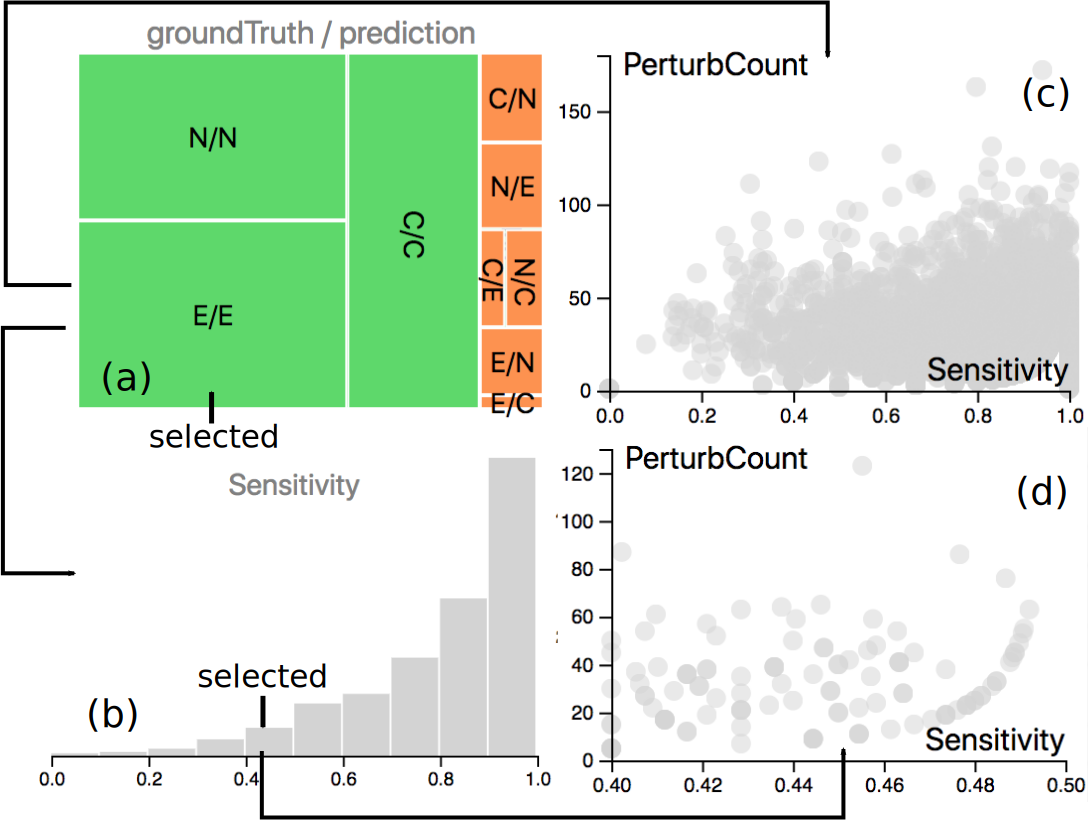
\includegraphics[width=1.0\linewidth]{summaryView}
 \caption{
Summarize the prediction results and sensitivity of the entire development set, and provide an explorative interface to select example of interests.
We summarize all the prediction results in (a), where the green block indicates correct predictions, and orange block indicates wrong predictions, and the label (e.g., E/E, E/N) indicates the ground truth label and the predicted label (N-Neural, E-Entailment, C-Contradiction).
%
The user can select the treemap to focus on the specific type of scenarios and reveal the histogram (b) and scatterplot (c) for displaying per-pair information on the selected subset.
The selection can be further narrowed down by select the bin in the histogram.
In (c) and (d), each point corresponds to one prediction.
 }
\label{fig:summaryView}
\end{figure}

%The all pair
% \begin{itemize}
% \item How to go from 10k pair to one pair
% \item What constitute interesting example
% \item How to get a sense of overall prediction result
% \end{itemize}
